Aufgrund einer Kopplung der beiden Gleichungen \ref{enq:Bewgltrans} und \ref{enq:Bewglrot} entsteht eine sogenannte algebraische Schleife, die besagt:

\begin{center}
	Ursache gleich Wirkung gleich Ursache.
\end{center}

Durch eine Vereinfachung des Systems soll die algebraische Schleife verhindert werden. Dies wird mithilfe von Matlab SIMULINK durchgeführt. \\
Die Parameter werden mit den Funktionen \ref{enq:Spannungen}, \ref{enq:Bewgltrans}, \ref{enq:Bewglrot} und \ref{enq:Unwuchtkraft} in einem Blockdiagramm verknüpft. So vereinfacht sich zum einen das System, zum anderen kann man leichter eine Aussage über das Verhalten des Systems treffen.

\begin{figure}[hbt]
	\centering
	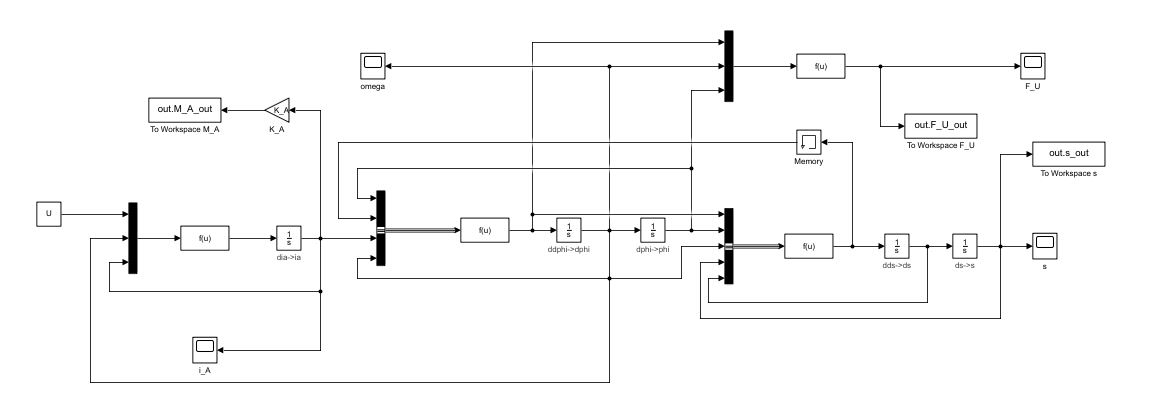
\includegraphics[width=1\linewidth]{Images/ProjektB_Elektrik_Blockdiagramm}
	\caption{Matlab SIMULINK Blockdiagramm zur Simulation des Systemverhaltens mit Memory-Block zur Umgehung der algebraischen Schleife}
	\label{fig:Blockdiagramm}
\end{figure}

Mithilfe von Scopes werden nun die gesuchten Signale abgegriffen und als Funktionen der Zeit dargestellt. \\
In der folgenden Abbildung \ref{fig:Simulationsergebnisse} sind Winkelgeschwindigkeit $\Omega$, die Strecke $s$, der Strom $i_A$ und die Unwuchtkraft $F_U$ über die Zeit von $100 \milli\second$ dargestellt.

\begin{figure}[hbt]
	\centering
	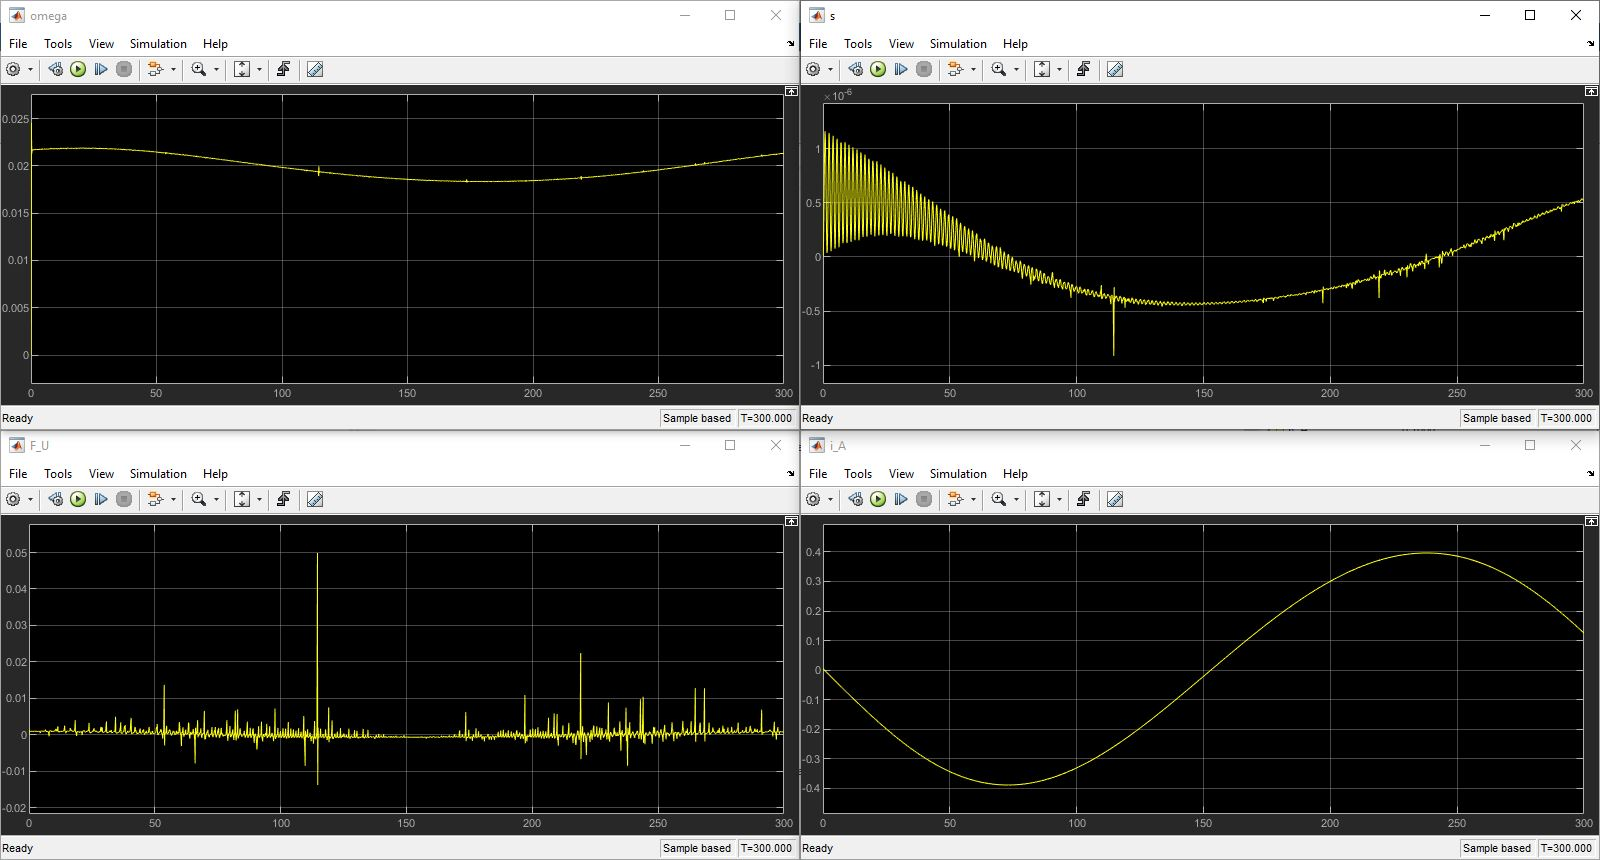
\includegraphics[width=0.5\linewidth]{Images/ProjektB_Elektrik_Diagramme_1}
	\caption{Ausgabe der Winkelgeschwindigkeit $\Omega$, Strecke $s$, dem Strom $i_A$ und der Unwuchtkraft $F_U$ über die Zeit von $100 \milli\second$ durch Scopes}
	\label{fig:Simulationsergebnisse}
\end{figure}
